\documentclass[11pt]{article}
\usepackage{lipsum}
\usepackage[margin=2.5cm, includefoot]{geometry}
\usepackage{fancyhdr}
\usepackage{verbatim}
\usepackage{graphicx}
\pagestyle{fancy}
\begin{document}
	\begin{titlepage}
		\begin{center}
			\line(1,0){300}\\
			[0.25in]
			\huge{\bfseries To Create and Compare the Predictive Accuracy of a Genetic Program and an Artificial Neural Network to Predict Corporate Bankruptcy: Final Report}\\
			\line(1,0){300}\\
			[1.5cm]
			
			 \textsc{Carl Saptarshi}\\
			 \textsc{\large  Student Number: 640032165 \\
			 April 2017}
			 
		\end{center}
	\end{titlepage}

\tableofcontents
\thispagestyle{empty}

\cleardoublepage
\setcounter{page}{1}
\section{Background and Introduction }\label{sec:intro}


Due to the dynamic and volatile economy that we live in, the number of companies filing for Corporate Bankruptcy (CB) are rising, especially in times of economic uncertainty, for example, during a period of recession. In turn, being able to predict the likelihood of a corporation going bankrupt and filing for bankruptcy is very important and has been a focal point of issue in accounting research and analysis over the past thirty years\cite{?}. 

\subsection{Background into Bankruptcy}
\subsubsection{What is Bankruptcy? }\label{sec:bankdef}
When a company (the \textit{debtor}) takes out a loan or borrows money from somewhere like a loan company(the \textit{creditor}) , it is up to the debtor to ensure that the creditor is repaid the full amount that was borrowed subject to the creditors terms and conditions.


If the debtor starts to fall behind on their payments and are unable to repay their debts, the debtor may file for a Chapter 7 bankruptcy in which the court will appoint a trustee to shut down the company and liquidate their assets, for example, by selling machinery, land and company shares to recover some money which they the trustee can give back to the creditor to clear the company's debt. If the company is still unable to pay back the debt even after this, the company will be terminated. As economies have grown rapidly since 1960's, especially in the western part of the world, bankruptcy has been recognised on a much grander scale\cite{?}

\subsubsection{Who does it Affect?}
Bankruptcy does not just affect those that are employed within that company; it also affects third party members such as shareholders, investors, and company clients. CB has been an area of interest, especially in the field of financial analysis and for stakeholders who are interested in the performance of the company\cite{?}. Since the 1960's, empirical risk assessment models have been developed which have been used to predict CB. 

Using financial data of a company, the likelihood of CB can be predicted for \textit{'n'} number of years ahead. 
Loan companies can use this information to determine whether loans should be granted to a corporation, as they will know the likelihood of a company defaulting or not\cite{?}. This has helped to give banks competitive advantages, as they become aware of how likely a company will be to default, and is able to predict customer behaviour in times of difficulty\cite{?}.

Looking at reports from the American Bankruptcy Institute showed that in the year 2000, 35,742 companies filed for bankruptcy, 43,546 companies in 2008 and 60,837 by 2009, at the peak of the recession. By 2012 this fell to 40,075 and 24,114 by 2016\cite{?}. These statistics clearly indicate the volatility and uncertainty in the economy as it changes, which is part of what makes CF prediction incredibly important.

\subsection{Algorithms for Corporate Bankruptcy Prediction}
As the aim of the project to classify whether a company is likely to go bankrupt, this type of problem can be called a binary classification problem. This takes a series of inputs and returns a classification which determines whether or not a company is financially distressed. Companies likely to suffer from financial distress will have certain characteristics associated with them, similarly for companies not facing this problem. This means that the data being used should be linearly separable when classifying the data, making this a linear binary classification problem. There have been several techniques that have been used to predict CB, some of which will be introduced here.  

\textbf{Individual Ratio Selection (IRS)} -In the 1960's, Beaver introduced IRS\cite{?}. This process involved selecting 30 financial variables, and converting these to ratios. Based on a threshold for each variable, this would determine if a company is financially distressed or not.

\textbf{Multivariate Discriminant Analysis (MDA)} - Altman created this technique in the 1960's, which takes uses a discriminant function to score a company\cite{?}. This function uses five financially weighted ratios. Based on the overall discriminant score, the company can be classified as financially distressed or not.

\textbf{Supervised Learning (SL)} - Some of the current methods to predict CB fall under the umbrella of Machine Learning (ML). ML is a form of Artificial Intelligence that allows a computer program to learn without the use of explicit programming\cite{?}. This means whilst the program is running, it will start to determine patterns in the data, and adapt the program appropriately to try to produce the best predictions and classifications.
In SL, the output after each iteration of each model is compared against the already known desired output. This can then be used for checking the model's classification accuracy. For every iteration, the model will start to learn, so the classification accuracy will start to improve over time. Eventually, when an unknown set of data (hold out data) is inputted into the model, it will be able to correctly produce an output to declare if the company in question will go bankrupt or to a certain degree of accuracy.

\textbf{Genetic Programming (GP)} - GP's are inspired by Darwin's Theory of Evolution and are a type of genetic algorithm\cite{?}, used for prediction and classification. A population of functions is created where fitter individuals in the population are more likely to survive and produce offspring that are (in theory) more suited to their environment. The aim of this is to create an optimal function which can give the most accurate classification prediction on unknown data to see if a company is likely to go bankrupt within one year. 

\textbf{Artificial Neural Networks (ANN)} - Also known as the Multi Layer Perceptron (MLP),  this technique is inspired by the interconnectivity of the brain and applies this to prediction and classification\cite{?}. ANN's are made of an input layer, hidden layers and an output layer which produces a classification based on the input. The network uses the weights on its neural that connect each node to the next layer, which are tweaked, based on the accuracy error, to allow the network to learn and give an accurate classification for unknown data. 
\subsection{Motivations For this Project}
At present, it is possible to extract copious amounts of historical financial data from a range of small, medium and large companies. Through looking at some of this data, we can see whether or not a company has declared bankruptcy or not as yet. Unfortunately, there is not an easy way to identify just from looking at the raw data, as to whether a company is financially distressed and the likelihood of the company going bankrupt in the foreseeable future. By selecting the most appropriate key performance indicators (KPI's) - financial variables that are known to affect a company's performance the most - this data can be manipulated and combined in various ways to help find a way to predict how likely a company is to go bankrupt and whether they are financially distressed. The combination of these KPI's should be classify any sized company. \\
In the past, several SL methods have been used to approach this problem. As seen in section 1.2, ANN's have been used to try to solve this problem. Whilst ANN's are known to have strong classification prediction accuracy to see if a company falls into the category of "likely to go bankrupt" or "not likely to go bankrupt ", ANN?s fail to provide is a mathematical formula that a company could use to enter their own data to see if they are financially distressed or a clear way as to how the model came to this classification. Altman provided a solution that worked very well for the state of the economy at that time \cite{?}, however as economies have changed over the years, Altman's discriminant function may not necessarily be the most optimal equation to use anymore. \\
A GP can be used to generate and evolve mathematical expressions to produce a function that can be used to classify whether a company is financially distressed and likely to go bankrupt in a user-friendly way, rather than just giving a prediction. This can also show which KPI?s influence a company?s performance more than other KPI?s.  \\


In this report, I will be discussing how I created an ANN and GP to predict CB. I start by introducing some of the research that was conducted to gain a deeper understanding of what this project entailed. Using this research, I then discuss the requirements that were needed to complete the project. When talking about ANN's, assume that the ANN structure follows the format \textit{(input, Number of nodes per layer, output)} format. Using this research, I then formulate my design specification which was used to form the structure of the models that were implemented to test the predictive accuracy of the two models. After this, I will go on to talk about how the models were tested individually and compared against each other, before giving an evaluation of the project that has been completed. After this, I will then mention some of the work that could be completed in the future to potentially improve this project, before coming to final conclusions. 
\newpage
\section{Summary of literature review and specification}\label{sec:spec}
\subsection{Literature Review}
All the techniques mentioned in section 1.2 have been used extensively in the area classification and prediction. Altman and Ohlson\cite{?}, pioneers of CB prediction since the 1960's selected financial variables from multiple company's bank statements to predict CB. These variables (\textit{key performance indicators} (KPI's)) were used as they believed these were important factors that indicated a company?s performance. To make companies more comparable, both techniques involved converting the KPI's into ratios as a method of standardising the data. Newer models proposed are based around Altman?s financial ratios and use their prediction accuracy for MDA and IRS as benchmarks to compare their new proposed work against techniques already in use. \\

Overall, Altman's model was superior to Beaver's method, but only if the KPI's were jointly distributed according to a multivariate normal distribution\cite{?}. Otherwise, it was prone to errors. However, the MDA technique was favoured as it could use multivariate data at once to get an overall prediction rather than taking each ratio and scoring that to give predictions\cite{?}. \\
Wilson \cite{?}and Lensburg\cite{?} used newer approaches by implementing ANN's and GP's respectively to this classification problem. Both of these techniques can handle noisy data that is unevenly distributed better than Altman's MDA, showing that both ANN's and GP's have potential to be more accurate than IRS and MDA. 

ANNs tend to perform very well in terms of performance and accuracy. Wilson et al used an ANN approach with a (5, 10, 2) structure\cite{?}. To improve predictive accuracy, the Monte-Carlo technique was used to give a better representation of classifications. Overall, they achieved a 97.5\% accuracy on their testing dataset, making this much more accurate than MDA and IRS. \\
Lee used a decision tree (DT) method to predict CB\cite{?}. Lee used 8 different KPI's when approaching this problem. Using this GP model, the testing accuracy of 92.91\%. Rostamy\cite{?} used a similar approach to Lee, using five different KPI's. After training the GP, it could correctly predict if a company would go bankrupt or not 90\% of the time, which was like MDA, however more flexible in terms of the type of data that could be used.

GP's may work slower as they explore a large search space and may be restricted to certain limitations e.g. a maximum tree depth. For each crossover and mutation, the depth of tree may increase. This can increase the computation time rapidly. When designing and implementing the GP, these factors will typically be accounted for as seen in Etemadi's et al paper\cite{?}. \\

Through the research completed, many papers used Altman's KPI's as their inputs. However, as Altman suggested, these ratios may not necessarily be the most optimal, but these still provided the best alternative discriminant function to work with at the time\cite{?}. Since then, economies have changed significantly, these ratios may not necessarily be the best to use to predict CF, but may still be significant enough to give an accurate enough prediction. As seen by Back, Rostamy and Lee\cite{???}, other ratios have been used to predict CF, and achieved similar results to MDA, which could potentially be more significant now. Wilson used Altman's KPI's and achieved the 97.5\% accuracy, with far fewer ratios relative to Back and Lee, which must be taken into consideration\cite{?}.
\subsection{Project Specification}
After careful consideration of the researched techniques, I will be predicting CB using ANNs and GPs due to their strong predictive accuracy rates and ability to handle noisy data. Though they do have drawbacks, I will aim to minimise these through the project specification and implementation.\\

As the models used in the research depended on various datasets, the first thing that needed to be acquired was a dataset with an enough data, and containing enough variables that could give an indication as to whether a company went bankrupt or not. The decision to use only small to medium enterprises(SME) was to have more consistent, comparable data, as shown by Altman. Using this dataset, I would then able to create financial ratios which can then be used in the models to be developed. 

Two programs were intended to be made for this project; a feed forward ANN with back propagation and secondly a regression tree GP.  I have chosen to take forward these two models is that ANNs are known to produce very accurate results efficiently. The reason a regression tree GP has been put forward is because this a valid technique that can be used as they are able to produce a function that will directly map the input KPI?s to give a classification.\\
Both techniques should give an indication as to which KPI?s affect the classification prediction, and give an indication as to which KPI?s affect the companies and could be a cause of their failure.  \\
As this is a binary classification problem, the output of each model determines whether a company can be classified as likely to go bankrupt or not. To represent the classification,  0 will represent a company that is not likely to go bankrupt  and 1 will represent a financially distressed company.

Since this representation is a number, the actual floating point value of the output (which will be between 0 and 1) for the NN, this number will be used to represent the likelihood of failure as a probability. For example, if the value was 0.618, it could be said that the company has a probability of 0.312 of staying afloat for the forthcoming year. Whereas if the value was 0.111 then the company has a 0.899 probability of staying afloat for the forthcoming year. Here, a clear differentiation can be made between two companies, one which is more likely to fail than the other.
Once the development part of the project is complete, I planned to test the results of both models, individually against each other to compare their predictive accuracies, and against Altman?s benchmarks results.

To allow the ANN to learn, I will be using the training dataset. When testing this, I will use a testing dataset to validate the results to see the true accuracy. I will also use K-Fold Cross-Validation techniques to help improve the comparability and the accuracy as well. On top of this, I will also be testing the data using the 50:50, 80:20 and 90:10 non-failed: failed as part of the training and testing of the data. To increase comparability, I will also use the same datasets for both ANN and GP.

I will also consider the number of iterations that have been used to complete the task in both ANN and GP. The time it takes to process the inputs will also be compared. To determine what KPI?s have a greater contribution than others, for the variables that are being used for ANN?s, I will remove one ratio, rerun the programs under the same training and testing conditions to then check the outputted value to see how significantly different the output is with and without that ratio. This will help to determine what ratios have a greater weighting and could be a significant factor in the future success or demise of a company. 

Overall, to make my project successful, I will take these factors into account before starting to program, to prevent any long-term errors that could occur. I will also use a reliable GUI to help prevent programming errors, which in turn will make my project more successful. 
\newpage
\section{Design}
For this task, two different models had to be designed and created as stated in section 2.2. Due to the size of this project, by breaking each of the models down into smaller, more manageable parts, it gave a better, clearer structure to how the two models would eventually be implemented through code. 
\subsection{Data Collection}
Before staring the design of the GP and the ANN, the first thing to do was to collect all the data that I planned to use. The data that collected had been given to me by the University of Exeter Business School as they had easy access to multiple year's worth of data for hundreds of companies. Due to the fact that each economy is different financially, and companies may perform better or worse in different economies, to make the data more comparable, the data that I collected was solely from American companies from the US economy.\\
The data collected contained 671 rows of data, with 31 different variables. For this project, only eight of the 31 variables were financial variables that were indicators of a company's performance. For example, \textit{net income} and \textit{sales} would be considered to be variables that could affect the company performance, however variables like \textit{company name} and \textit{ticket}, would be much less likely to affect the company's performance. Therefore, to make the data more usable, variables not considered to be KPI variables were removed from the dataset. After completing this, the next step was to remove incomplete data. Some of the rows of the data contained question marks (?) where cells were missing data. As this could have potentially affected the programs and how the data is read in and make the data harder to work with, any rows with any incomplete data were filtered out. Now the dataset contained only complete data with the key financial variables. Due to the types of the companies being given, to make smaller companies more comparable to larger companies, the next step was to standardise these variables into five ratios, similar to the methods that Altman used to standardise his dataset. This new standardised dataset contained five variables, labelled X1, X2, X3, X4, X5, each representing a specific ratio, and finally the classification for that particular row, to indicate whether or not that particular company had failed or not, indicated by a 1 for failed, and a 0 for not failed. Since this dataset was now in the right format, the next stage was to design the GP and the ANN that I chose implement. 

\subsection{Artificial Neural Network Design}
Now that the data collection process had been completed, the next step was to design the ANN. After completing the relevant research, the type of ANN I chose to implement was a feed forward artificial neural network. The reason that this was chosen is that based on the research that was undertaken, the papers that implemented an ANN used a simple feed forward network as this avoided any unnecessary complexity that would occur if other types of ANN's were used. An ANN usually follows the same layout which makes them applicable to an array of complex problems. The basic structure of the ANN consisted of an input layer, hidden layer(s) and an output layer.
\subsubsection{Input Layer and Synaptic Weights}
Now that the dataset had been modified into five KPI's and a classification feature, I had to decide what the input features would be used for this network. Since ANN's are able to cope with high dimensional, non-linear data, I decided to use all five of the KPI ratios that I had created from the dataset as the ANN would be more than capable to handle all the data that I was planning on giving it.\\
Due to the stochastic nature of an ANN, when initialising the network before the data from the input features are read into the network, the weights that each node in the previous layer to each node in the next layer also needed to be initialised. As part of the design, I chose to completely randomise the weights on each of the synapses. If the weights were not initialised randomly, when the network starts to learn, it would learn in the exactly same way every time the program is run because the network will always start at the same position in the search space, which means it will always follow the same route to get to a solution which would always be the same since the stochastic element has been removed.  By initialising the weights randomly, the symmetry of the network is broken, which allows the network to be initialised differently, so the weighted input signal that moves from one layer to the next would always be different, allowing more of the search space to be explored, which would allow more solutions ( possibly more optimal solutions) to be found. 
\subsubsection{Hidden Layers and Activation Function }
The next step is the structure of the hidden layers of the network.  For this, I have decided to use two hidden layers with between 1-100 nodes. Through research, it was found that a sufficiently wide ANN with just one hidden layer would tend to be enough to train the ANN without memorising on the network. However, the wider the network, the more likely it is that the network will be to memorise the data, which means generalisation will be poorer, such that although the data has learned well when training the network, the accuracy when testing the network would be poor as the network has overfitted the data. Therefore to attempt to avoid this, I will use two hidden layers as this would allow the network to generalise better without network memorisation. Rather than using trial and error, I decided to use cross validation to find the most optimal number of nodes for each one of the hidden layers. To do this, the network would be cross-validated 5 times. The reason cross validation works is that it will attempt to perform all the permutations of the nodes on the network with the intension of finding 'n' number of nodes in the first hidden layer and 'm' number of nodes in the second layer which would result in the best training accuracy. Once these have been found, this network can then be tested on by using the testing set of data. \\
\\
At every hidden layer node, the weighted sum of the input to that node will be calculated. This weighted sum will then be passed through an activation function which will then send the output of this node to be the input to the next layers nodes. For the simple ANN that is being designed, I will initially use a sigmoid activation function. The reason this is a good idea and should be part of the design is that the sigmoid function adds an element of non-linearity to the to the model, which allows the computation of nontrivial problems using only a small number of nodes, which is what makes this particular function much more popular relative to other activation functions like a step function. 
\subsubsection{Output Layer and Learning Mechanism}
After the input has been fed forward through the network, the output will be produced. When training the network, I will classify the outputs as either a 0 or 1 by passing the raw value through another activation function. If the value outputted is below 0.5, then it will be classified as a 0, otherwise it would be classified as a 1. Using this, the error percentage can then be measured against the true results, and the weights will be altered accordingly using a learning mechanism. For this network, through the research conducted, the back - propagation learning method should be sufficient enough to allow the network to learn, to try to minimise the error rate, to give the best possible accuracy, showing that the network has trained.\\
Once the ANN has produced an accuracy of 80\% or higher on the training dataset, I will then use a testing dataset to test the predictive accuracy of the classifier on unknown data. This process will occur multiple times during the process of cross validation as the network will be selecting various weights and number of nodes with the aim of producing the most optimal network within a sufficient amount of time.

\subsection{Genetic Program Design}
\begin{figure}[h]
\centering
\includegraphics[scale = .37]{GPFlow3}
\caption{Figure1: Flow chart to represent the Genetic Program that has been designed} 
\end{figure}
As the ANN had now been designed, it was ready to now be implemented. To see the implementation of the ANN, please refer to section "Development of ANN". The first stage in the design process of the GP was to consider the data structures to be used. Since the solution to the GP will be an optimal function consisting of a mathematical expression, the easiest way that this could be represented is using a binary regression tree. The reason that a binary tree was chosen is because in genetic programming, when using a tree structure, it enables for crossover and mutations of subtrees and nodes to be significantly easier than if using something like multiple lists. Not only would that be more computationally expensive, but the expressions generated would be much harder to read from a users point of view. As part of the regression tree to be made, each node in the tree would need to consist of either a functional value e.g. a mathematical operator (making this a branch node), or a terminal node e.g. a variable or numerical value (making this a leaf node). When approaching the design of the tree structure, the first thing I accounted for was the functional set of values. I chose the four core operators: [+,-,*,/] due to the fact that they maintain the same arity of 2.\\
 Next I decided to use all of the 5 KPI ratios for my inputs, as these were going to also be the same inputs for the ANN. The 5KPI's and a random floating point value between 1 and 50 made up my terminal set of values. Now that this was done, the next step was to think about the representation of each of the stages of the genetic program that would eventually be implemented. 
 
\subsubsection{Generating a Population}
Looking at figure 1, the generation of the population is indicated by the green boxes. For this part of the project, the aim is to try to create an optimal function, which would be an optimal mathematical expression that a user could use by inputting their own data which would determine the likelihood of the company failing within one year. Since the goal is to make an expression, when generating the population of individuals, I will use a random expression generator to create these. When doing this, two things will have to be taken into account. The first is since all the input features are going to be used, each member of the population should contain at least one of each of the input features from the terminal set to ensure that all of the input features are being utilised. Secondly, the depth of the tree must also be taken into account. This is because as trees grow, the computation time to evaluate and use them will increase, therefore to prevent very large trees initially, a depth limit will be set as the trees will get larger through the process.   Next based on the research that I have done, I will use a population size of 500 individuals.
\subsubsection{Fitness Function}
Indicated by the blue boxes in figure 1, the next step is to evaluate the fitness's of the individual expressions in the population. For this I will use the Number of Hits fitness function whereby the data that is passed in will evaluate to a number which will either be a negative or positive number based on the expression being used and the data being passed into the expression variables X1-X5. If the value is positive it will be classified as a 1, otherwise it is a 0. Using the class labels from the data set given, I can then compare the predicted classifications to the actual classifications. If an expression produces many mismatches between the predicted output and the actual classification, the expression should be given a worse fitness value, otherwise give the expression a better fitness value, where the best possible fitness value would be 0, if the expression was able to correctly classify every single row of data. 
\subsubsection{Selection}
Once the population has been generated properly and the fitness of each of the members have been evaluated, the next step is to select the parents that may be put forward for the genetic operations; crossover and mutation. To select the parents, I have chosen to use tournament selection. This works by selecting a random subset of the population, \textit{t}, and then comparing the fitness's of each of members of \textit{t}. The individual with the closest fitness value i.e. closest value to 0, will be selected to be the first parent. This same process will occur to select the second parent, however as part of this, each individual can only be selected once per generation, the same member of the population cannot be selected as both the parents. 
\subsubsection{Crossover and Mutation}
Now that the two parents have been selected as expressions, children now have to be created. This can be done by the processes of crossover and mutation (indicated by the orange and yellow boxes respectively). To begin with, I decided to use a lazy instantiation approach, whereby I have to convert the infix expression into the binary tree as this will make the process of crossover and mutation easier. The reason I chose use lazy instantiation was because it would save computation time from having to generate binary trees for every single expression, even though only two members of the population will be going through the genetic processes to create children. Once the two parents have been converted into binary trees which consists of multiple nodes, the next step would be to select a random subtree in each parent, and then perform the single point subtree crossover which will create two children, each containing parts of both parents. \\
After the two new children have been selected, another genetic operator can be used to alter the children slightly more. This is the process of mutation. Here, I will be using single point mutation, where a random node on each of the parents will be selected and that node will be altered based on its arity. For example, if the node selected is a numerical value, with an arity of 1, then this will be replaced by another value with an arity of 1, and similarly if the node selected has an arity of 2, then it will be replaced by another functional node. 
\subsubsection{Termination Criteria}
The termination criteria will occur in two places as indicated by the red boxes in figure1. The first termination criteria is if an optimal expression has been found in the population. Since there is a possibility of this occurring when the population is generated, this should be checked before the program continues. If an optimal solution does exist, then return the best individual. If after 'n' generations of running the program, the best individual in the population still has not been able to meet the optimal fitness criteria, then the program should stop  and return the fittest individual in the current population as this has a fitness values closer to 0 compare to all others in the population.  \\
Using this expression that has now been returned, it should be tested on the testing dataset to check the predictive accuracy of the expression to see if it has predicted whether a company is likely to fail or not. Based on the output given, this should then be passed through a transfer function such as a sigmoidal function, as this will allow a value between 0 and 1 to be produced, which can be used to determine the probability of failure for that one particular company based on the testing dataset. 

\subsection{Choice of Programming Language}
The final part of the design stage was to determine what programming language that could be used for this project. Through careful consideration, I decided to choose Python as my main programming language. The main reasons for this were that since the ANN was going to be used as a benchmark, rather than trying to implement an ANN from scratch, I chose to use a library - sklearn, as this provided all the functionality to allow a feed forward ANN with back propagation to be created, along with many other functions which could be used to test the network e.g. using other transfer functions, methods of splitting the data and how to train and test the network. Since Python was what I was going to use for the ANN, for consistency, I also decided to use Python as the choice of language for the regression tree GP. This was because of the fact that Python offers object orientation, speed, high level abstraction for memory allocation and offered others optimised mathematical libraries such as Numpy which can make data handing easier, and Matplotlib which offers easy to make graphs which can then be used for data analysis.
\newpage
\section{Development}
Based on the design of the project, I was now able to start creating the ANN and the GP to predict the likelihood of CF within a one year period. To make the development more manageable, I decided to work on using smaller problems, with static data such that if issues did occur, debugging and understanding the errors would be easier. To make the testing phase more reliable, I decided to use the same dataset for the ANN and the GP. \\
Since the dataset was the same for both programs being made, I used the same method to read and split the data sets from their associated classifications. As this was a supervised learning problem, the decision to split the data was because the classifications from the dataset could be used to form the fitness functions for both techniques that were implemented. 

\subsection{Development of the Artificial Neural Network}
As the ANN being implemented was going to be used as a benchmark to test against the Genetic Program, rather than implementing the ANN from scratch, as part of the design stage, I chose to use a library in Python - Sklearn, a well known machine learning library that has the facilities to develop a feed forward ANN quickly, and the ability to train, test, and present the outputs of the data in a variety of ways.  

\subsubsection{Multi Layer Perceptron Classifier}
After the data set had been read in, the data was stored in a variable \textit{data\textunderscore CBD} and the classification labels were stored in a \textit{class\textunderscore labels\textunderscore CBD} variable. Since the data was read in using the numpy module, the data was kept in an numpy array, therefore to keep the data and classification labels types the same, I converted this list to a numpy array as well to avoid conflict later on. \\
\\
Now that the data had been read in completely and in the correct format, the main part of the program could now be implemented - making the ANN. To do this, using the \textit{sklearn.neural\textunderscore network} module, I imported the MLPClassifer. Using the MLPClassifier constructor, after the data has been fed into the network, I chose to use the \textit{logistic} function as my activation function as this is the most population activation to use on feed forward ANNs.\\
When creating the network, the weights on the synapses of the network are initialised randomly, such that the network can explore the search space differently each time, and aim to try to find the most optimal solution i.e. a network that has the best predictive accuracy and is able to generalise well so that it will handle hold out data, and not overfit the network.\\
To allow the synaptic weights to learn, there were different solvers that could be used to train the network. Since the back-propagation field was unavailable, I initially chose to use the stochastic gradient descent as my method of adapting the weights to train the network. Initially, as part of the constructor, I chose to have use the L2 regularisation parameter (the alpha parameter). A regularisation parameter is used to penalise networks that are more complex, as they are able to train networks better but have tendency to overfit the data, which means they will have poor regularisation, and therefore will have poor predictive accuracy when predicting on hold out data. Another parameter that was used was the momentum parameter. In the process of gradient descent, i.e. the way the network learns to find a better solution, the aim is to try to minimise the error function with the intention of trying to reach a global minima in this case. This is because we are trying to minimise the error to get the best possible predictive accuracy. Due to the nature of the data, there is a strong likelihood that the data will get trapped in a local minima and assume that this solution is the best, when in fact there may be several better alternatives. Momentum is used with the intension of increasing the size of the steps taken towards the minimum by trying to jump from a local minima. However, this parameter is invalidated when using any other form of solver other than stochastic gradient descent is used as momentum is only used in sgd. The final parameter used for the MLPClassifier constructor was the \textit{hidden\textunderscore layer\textunderscore sizes}. Based on the research conducted and as part of the design stage, I initially chose to use one hidden layer with five nodes within this layer. This particular structure was based on Odom\cite{?} ANN as this was an ANN that had already been used and worked. \\
As this entire network was able to run the ANN very quickly, I was able to run the neural network against my current dataset and get a result. Now that the ANN had been created, and could be used as a benchmark, I was able to start the development of the genetic program.

\subsection{Developing The Genetic Program}

Throughout the development of the implementation, to begin with, a sample set of data was used based on the actual dataset. The reason that this was done is so that I could get the structure right for when the actual dataset would be used. On top of that, throughout the development phase, rather than trying to tackle the main problem from the start, each of the parts of the development were broken down to be able to approach smaller problems which I knew would work, as debugging the errors became easier. After I was able to make smaller problems achieve the correct solutions, I started to work with more data with bigger trees such that I could handle any other issues that may not have risen whilst working with the smaller datasets and smaller populations, depths and time frames. 
\subsubsection{Reading Company Data}
To begin the process, I initially hardcoded static data from the initial dataset into my GenMember class. The reason for this was because whilst developing the program, using a small dataset made understand where the data is being use and when significantly easier as I was able to track the data as it went through the program.\\
After the program was fully created and working, I created a class called \textit{Data} which was used to read and split the data. The constructor used sets the file to be used, in which this file can then be used throughout this class. The second function to be made in this class is \textit{read\textunderscore data} which is used to read the data, and split the data into a matrix containing only the data columns X1,...,X5, and a column matrix containing only the data classification labels. These were then fed into the \textit{GenMember} which could now be accessed from anywhere within the program as the variables \textit{data} and \textit{labels} are static and therefore can live outside its scope.  
\subsubsection{Generating and Handling the Population}
The first stage in the development process was to create a population of expressions based on a maximum depth limiter and population size. To do this, I created a class called GenMember. The purpose of this class was to handle the current population by generating all the members, finding their fitness's, selecting the parents and updating the population.\\
The first function that was created, \textit{generate\textunderscore expression }was used to generate a random mathematical expression in infix notation using recursion and a maximum depth. The reason that recursion was used here is because this seemed like a logical way to generate the terminal values and variables, as well as to utilise the functional set. This function takes into account a maximum depth parameter. The reason for this is because as members of the population are generated, they will be generated in a variety of sizes ranging from an expression size of 1, to size n. As the size of the expression increases, the longer it will take to evaluate and manipulate the expression,  therefore to ensure that that the expression stays a reasonable length, a \textit{max\textunderscore depth} parameter was imposed. For every iteration that the function runs, the depth is reduced by 1, and once the depth is 1, a randomly selected value from the terminal set is selected. Eventually this will produce a random expression, which would be mathematically valid. The generation of the expressions have been based on Koza's ramped half and half method as rather than using a full or grow technique, as this provided more variety in the solution sizes, which makes these expressions more organic. Unfortunately, since not all of these expressions would  necessarily contain all five of KPI ratios, I created another function called \textit{get\textunderscore valid\textunderscore expressions}. This function was created to create the user defined population size, whilst ensuring that invalid expressions were filtered out and replaced with valid expressions.\\
\\
Now that the population of individuals have been generated the next function to create was the fitness function - \textit{get\textunderscore fitness}. This function is called in two different scenarios - when the population is initially created and secondly when the new child produced is to be entered into the population. When the population is initially generated, all the individuals need to be evaluated to find the fitness's of all the solutions as an optimal expression may exist within the original population. To evaluate the each member, each row of the sample data is fed into the population of expressions, and the total was found. If the value was positive, then the expression for that row of data would be classified as a 1, otherwise it would be classed as a 0. The actual data classification labels were then compared to the predicted classification labels. For every incorrect prediction, the fitness value would increase by 1, indicating a high level of error, therefore very poor solutions would have a very high fitness value, whereas very good individuals with strong predictive accuracy had a very low fitness value as the aim is to minimise the error, therefore they had a high predictive accuracy.\\

Since the population has been generated and the fitness's have been evaluated, the next step in this procedure was to create a function that would be used to select two parents in the population that could be to create the offspring. This method for this, as described in design stage, I decided to implement tournament selection initially.

To perform tournament selection, the population and their associated fitness's had to be inputted as parameters, as well as a user defined tournament selection size. This size refers to the number of individuals that would be selected randomly in the population, which would then be compared against each other, and selecting the individual with the best fitness to be the first parent. As the population and fitness's are read in separately, to save some time, I immediately zipped the individuals with their respective fitness's into a list of tuples using the zip function. Based on the \textit{selection\textunderscore size} selected, \textit{'c'} candidates were selected randomly from within the population.  Using these candidates, their fitness's are compared and the individual with the best fitness is selected to be a parent. 
After the first parent is selected, this individual is removed temporarily from the population to prevent the same parent being selected twice. This same process is repeated again to select the second parent, and finally both of these selected parents are then returned from this function. \\

\subsubsection{Infix to Prefix Conversion}
As the parents have been selected, the next stage of the development process was so convert the parents from its current state i.e. infix notation to another state called prefix notation, as this is easier for a computer to parse into a tree structure.  Currently the parents were stored as a list of strings e.g. [['1+X1'],['2+X2]].
To organise this part of the project, I put all the functions relating to this conversion into a class called \textit{ToPrefixParser}. In order to convert the parent infix expressions into prefix expressions, each element of the parents had to split up into individual elements. After this was completed, I appended the string 'stop' to the end of each parent as this will allow the conversion from infix to prefix to never go beyond the number of elements in each of the parent lists. One of the problems splitting the parents up into individual elements meant that variables such as 'X1' were split into ['X','1'], therefore to split an expression such as ['1+X1'], I used regular expressions 'w+' and 'W' to ensure that alphanumerical characters were kept together such that the new expression would be ['1','+','X1','stop'] which could be converted into prefix notation now. \\
Albeit when working with integers, this function worked well, when dealing with floating point values, when a floating point number such as '3.14' was part of the expression, this would be split up into ['3','.','14'], which caused the program to break. To work around this, issue, a function called  \textit{fix\textunderscore dec} was made, which would go through the split list, and wherever a decimal point existed, it was join the previous and next value relative to the decimal value, such that ['X3','+',3','.','14','stop'] would now be ['X3','+','3.14','stop'], which therefore split the lists into their correct form. \\
\\
Since the parents had been split correctly, they could now be converted into prefix notation. Using [insert website name here], I was able to find code which could be manipulated to enable me to convert the infix notation into prefix notation as this website was not sufficient enough by itself. The \textit{get\textunderscore operation}  function is used to compare the \textit{0th} element of the expression that is being passed in to the \textit{expected character} that the parser is looking for.
 If they match, then this value is popped out of the original expression. The \textit{expected character} is checked throughout the other parsing functions. The \textit{is\textunderscore number} function is used to return a number which is a leaf value. 
However if the character being checked is a "(" and the expected character is also a "(", then this will call the \textit{get\textunderscore expression} function which in turn would be used to get the subexpression that exists within the pair of parentheses. When  \textit{get\textunderscore expression} is called,  a chain of other functions are called sequentially, which will put the infix notation into prefix notation.
\textit{get\textunderscore expression} calls the \textit{get\textunderscore product} function, which then calls the \textit{is\textunderscore number} function which checks to see if the current character being checked is a "(", in which case the sub-expression is then evaluated, otherwise a number is added to the prefix notation output.  As each character in the infix notation is checked, these functions are called to correctly convert the infix notation into prefix notation. \\ 
After both parents have been converted from infix to prefix notation, the newly converted parents are returned by the \textit{get\textunderscore prefix\textunderscore notation} function.  
\subsubsection{The Node Object}
Since both the parents are now in their respective prefix notation formats, the next stage of development is to build the tree. A binary tree consists of two types of nodes; branch nodes and leaf nodes. Branch nodes have the ability to hold a value, and have "left" and "right" child references. Leaf nodes on the other hand can hold a value but have no child references. Both branch and tree nodes have parent nodes which can also be references. The top of a binary tree is called the root node, which is a branch node, however it is unable to hold a reference to a parent as it the eldest generation. Multiple nodes that are connected form a tree. \\
Based on this general structure of what a node can and cannot hold, I decided to make a class - \textit{Node}, which has four functions. The first function is the constructor which holds all the possible features that a node object could hold. These include the current node value, the possibility of holding references to a left and right child, the possibility of holding a reference to a parent node, and finally an ID field which assigns a unique number to each node as they are created such that two nodes with the same value in it are still different nodes and will be referenced to by their ID value, rather than the value they possess. Each node is null until a value is assigned to it, which will be done when the tree is being constructed. The second function that the Node class holds is the ability to add a child node. This function takes in a value and will either insert a child into the parents left branch or right branch depending on the state of the "left" parameter. Every time a new child is added, the child also holds a reference to its direct parent to indicate that the child is connected to that one specific parent. \\
The final two functions are used to give a visual text based representation of exactly how a tree would look, therefore for each level that the tree goes down, the child of a parent is indented accordingly. The root node will always be the first node to be printed out at the top and furthest to the left of the terminal window, whereas the deepest child will be printed furthest to the right of the terminal window. 
\subsubsection{The Tree Object}
Now that the parents have been selected, and the Node object has been created, the tree can now be built. As part of the design stage, I chose to perform lazy instantiation as this would save computation time by only creating a tree object based on the parents rather than creating trees for every member of the population, as only two trees will ever be manipulated at once. To begin with, the Tree constructor contained a root node, as this is how all trees need to begin, with a root node. 
Based the prefix notations, I was now ready to construct a binary tree for a parent. To do this, I created a function called \textit{make\textunderscore tree}. To initialise the tree with a root node, the first index of the prefix list was removed and assigned to be the root node. To enable me to track the nodes, I used a \textit{current\textunderscore node} variable which was initially set to the root node. Since this node has now been created, it was removed from the parent prefix list as it is no longer needed. Based on the current node that had been selected, I performed a check to see whether or not it was within the functional set of values. If the current node was a functional operator, then it has an arity of 2, which means that it would need to have exactly two children, a left and a right child. Therefore I perform to check if the left child for that node has been created. If it is empty, then the next value in the prefix list is inserted into the left child and the left child becomes the new \textit{current\textunderscore node}. If the current node is not a functional operator, i.e. it is a leaf node from the terminal set of values, then this cannot have any more children. In turn, go back up to the leaf node parent and check to see if the right node can be created. If it can, then continue construction of the tree via the right branch. Otherwise keep going back up the tree to the root node and then start building the tree to root node right child to build the rest of the tree. After each value in the prefix list has been assigned to a node and the tree is completely built, the length of the prefix will now be 0. As a result, the tree has now been built, so the root node can now be returned. The reason only the root node has to be returned is because the root node has access to all its children which is the full tree, so every node can be accessed from the root node. a list of nodes is also returned to return all the subtrees of the tree as this will allow accessing the nodes for crossover and mutation to be easier. Finally, another variable \textit{nodenums} is returned which is used to track the node ID of each node in each tree. As each node is created, it is assigned an ID value. I made the node id variable static such that regardless of what tree is made, the value of the ID will always increment by 1. The reason for this was because when performing crossover and mutations on the tree, I would not have to reassign the node ID's to the new trees, they could keep their original node ID's as each node ID is unique.
\subsubsection{Crossover and Mutation}
Through the process of crossover and mutation, two new children would be created, containing certain characteristics of both parents, but being unique in their own ways. Since I wanted to keep the parents in the population, and not directly replace them, before starting this process, I used a deep clone function to clone both the parents. The reason for this is by using a deep clone, the parent clones would be completely independent entities from the original parents. Using these parent clones, the children could then be produced, based on the parents characteristics. \\
\\
Once a tree has been created, looking back at the design stage, I chose to complete a subtree crossover. To perform the crossover, three functions were created. The first function was \textit{select\textunderscore random\textunderscore val}. The purpose of this function was using the list of nodes that were created when a parent tree was made, I could easily now select a random subtree from the list of possible nodes . By doing this it would mean that the node selected and its entire subtree would also be selected. When selecting the node at random, I chose to remove the root from this selection, as every node is a subtree of the root node, which means if crossing over occurred, then the full tree would be crossed over and this was prone to errors. By removing the possibility of the root node being selected for cross over, this error was overcome. This function returned the node that had been selected as well as the node's unique ID. \\
After the specific node had been selected, to ensure that the subtree did in fact did exist in the tree, I created a method - \textit{find\textunderscore subtree} which was used to locate the subtree within the parent. This function took three parameters. The first one was the tree itself as this is what would be searched, the second parameter was the list of nodes as this is where the random value had been selected from and the random subtree would be selected from this. Finally the last parameter to this function was the random node ID that had been selected. Due to the way that the tree was created, each node was assigned based on a depth first creation of the parent tree. Therefore, to search for the subtree within the parent, I chose to implement a recursive depth first search. If the depth first function located the node value, it would then also check the node ID to ensure that this was the correct node to be selected. Checking the node id was necessary to ensure that the correct node was selected as there was a possibility of two different nodes in different parts of the tree having the same value. However as the node ID's were unique, there could only be one of each. If this termination criteria was met, then the subtree was returned. However if the node chosen was not in the list, then an error is through to indicate that the depth first search was unable to find such a node with that specific node ID. However this should never happen as for crossover to work, the node selected from the list of nodes needs to be within the parent tree this subtree of the parent will be crossed over with the other parent. \\
Once the subtree has been selected from both parents, I then created another function called \textit{swap\textunderscore nodes}. The purpose of this function was to simulate genetic crossover between the two parent nodes as this is what would create the children. This function took four parameters, including both the parent (clone) trees - which would be updated during the process of the crossover, and the nodes selected to be crossed over with each other. This function first gets the nodes selected parent node and performs a check to see whether the parents child is its left or right child, which is the node to be crossed over. By doing this, it is ensured that the correct subtrees are being crossed over with each other. Once the nodes have swapped over, the first parent now contains the second parent subtree and vice versa. \\
Once the crossover had been performed, the parent clones were now considered to be the children of the original parents as each new tree contained characteristic from both parents. As crossovers are more likely to cause bigger changes when searching the search space for an optimal function, it was recommended that crossover does not occur during every single epoch. Therefore I used a crossover rate which can be defined by the user as a value between 0 and 1, where the user can select how frequently they want crossover to occur. After the new children have been made, they move onto the next stage which is mutation.  When the cross over rate is low, there is a greater likelihood of crossover not occurring. When crossover does not occur, the parent clones remain exactly as they are and will progress to the next stage of mutation unchanged. \\

Although the parent clones were updated to produce the new children trees, the list of nodes that they each possess had not been updated. Therefore before children could be used for mutation, which uses the list of child nodes, the children had to have a list of nodes that they could each have as well, similar to their parents. To do this, a function called \textit{make\textunderscore list\textunderscore nodes} was created, to use the child tree and build a list of nodes which could then be used for mutation. \\
Once the list of nodes were built for the children, the process of mutation could now begin. Similar to the process of crossover, I used the \textit{select\textunderscore random\textunderscore value} function to select a random node that would be selected for the mutation. After this node was selected, the node was then found using the \textit{find\textunderscore subtree} function. Next, the \textit{mutate\textunderscore node} function was created. This function took into account the tree to be mutated, the list of nodes it held , the node to be mutated and the new fitness of the child. This function checks to see what type of value has been selected to be mutated, i.e. whether it is a functional node,  a variable node or a numerical value. If the value is from the functional set, then it will randomly select another value from the functional set as they all the same arity. However, if the value is from the terminal set, then another check is performed to see if the value is a variable X1,..., X5 or a numerical value. If the value is a numerical value, based on the fitness of the child, the mutation will cause the node to be altered by a certain amount. However, if the selected node is a variable, then it will randomly select another variable instead. Whatever value is mutated automatically updates the tree and updates the list of nodes accordingly to ensure that the newly created child is consistent with all the changes that have occurred. Similar to the crossover rate, mutations are not meant to necessarily occur during every epoch, therefore a mutation rate was used, which again, will be defined by the user, however by default is set to 0.1 such that mutations would only occur 10\% of the time. 
\subsubsection{Prefix to Infix Conversion}
Once the children have been made, they need to be evaluated such that they can then be compared against the original population and potentially replace the worst members in the population. To be able to evaluate the children, the children had to be converted back into infix notation such that the \textit{get\textunderscore fitness} function could be called. To do this, I created a class called \textit{ToInfixParser}. \\
\textit{ToInfixParser} contained two methods, which would convert the tree back into infix notation. The first function, \textit{deconstruct\textunderscore tree} takes each of the nodes from the child list of nodes, and extracts each of the values from the list of nodes, to return it back into the prefix notation state. The second function, \textit{conv\textunderscore infix} takes the prefix list, and goes through each of the values in the prefix list, starting from index -1. For every value that is not an operator, it adds the value to the stack. If an operator is encountered, it pops the values currently into the stack and puts the current sub- expression into a bracketed form - '(<operand1><operator><operand2>)'. This starts to build up the full expression back the infix notation, which is now in a state that the original population will accept. Finally, since the expression will be in the form '(infixexpression)', the first and last parentheses are unnecessary, therefore the first and last parentheses are not included in the output as they do not affect the output.


\subsubsection{Updating The population}
As the new children that have been created have been converted back into their infix notation, the next step was to find the children fitness's, using the same \textit{get\textunderscore fitness} function. However,  since this is a child expression, when \textit{get\textunderscore fitness} is called, the default \textit{child} Boolean variable changes to true, such that the child expression is parsed into an acceptable format that will allow \textit{get\textunderscore fitness} to return the fitness in the same state as if the population was originally evaluated. \\

Once the child fitness's have been found for the children, the population can be updated accordingly. To do this, the function \textit{update\textunderscore population} was called. This function takes the original population and the new child, and compares the new child against the worst member in the current population. If the child is better than the current worst member of the population, then the child will replace this member in the population. This process is repeated for the second child as well, to ensure that the worst members of the population are filtered out, and to enable the GP to start learning, but accepting better fitted individuals and rejected those that are worse. By replacing one individual at a time, this also help to make sure that the population size remained the same size as when it started. 
\newpage
\section{Testing}
Through out the development of the ANN and the GP, I used various methods to test whether the code was performing the way it should, and to see if different techniques affected the training and testing predictive accuracy of both the models. For both classification models, before being able to run tests on the implementations, I created a testing plan which was split into two sections for both models. The first section of the plan related to testing the code functionality to check whether or not each function was performing as it should which would lead to the correct outputs. The second section of both plans related to testing whether or not the programs made were definitely classifying the data appropriately and to change various parameters to see if this affected the training and testing predictive accuracies.\\
In this section, I will be discussing the methods of testing that were completed for the ANN and the GP for each of these two sections. 
\subsection{Code functionality \& Parameter Tuning: Artificial Neural Network}
Since the feedforward ANN was created using a library which is a very well known library for machine learning, it did not seem necessary to test whether or not the function to create and run the ANN worked the way it should. The reason for this is that through reading the documentation of the code, it can be seen that the classes and functions available have been thoroughly tested before being deployed to the public and are made to be user friendly. \\

On the other hand, even though code testing did not have to be done, there were still many different ways that the data could be used in the model which would give different predictive accuracies. \\
After reading in the data, I decided to split the data up into two sets. Training and testing data. The training data would be used to train the ANN by altering the parameters of the synapses, and the testing data would be used to predict how accurate the model was on unknown hold out sample data. By doing this, it means that the network is able to train on one set of data, and the performance of the model can then be evaluated based on the testing data. The benefit of using the train test split is that the testing accuracy rewards simpler models, rather than overly complex ones. After the data was read into the program, the data was shuffled to begin with to be the data. The data was shuffled to reduce the bias of selecting more rows belonging to one classification than another, therefore every row has a more equal chance of being selected. To split the data, I used the \textit{train\textunderscore test\textunderscore split} class. Within this constructor, I chose to use 80\% of the data to train the model, and 20\% of the data to test the performance of the model. For the ANN, I used one hidden layer with 10 neurones in the layer. After training, the predictive accuracy based on the trained model was 72.57\%. After rerunning this multiple times with the same variables, the predictive accuracy changed each time. The reason for this is because the testing accuracy has a high variance estimate. What this means is that every time a new set of data is being used to train and test the data, since this is random, the network will train differently everytime it is run as the observed values in the training set will differ each time. This is one of the biggest drawbacks of this particular method. \\
\\
One way that this problem can be overcome is by using another method - \textit{K-Fold Cross-Validation}. Cross validation is essentially the idea that the train test split method is run several times, using different train test splits, calculating the testing accuracy each time and then taking an average of all the results to get an average prediction, which in turn would also reduce the variance. For this to work, the data is divided into K partitions, where one set would be used to train the model , and the rest of the data is used to validate the model, calculating the predictive accuracy each time. This process is repeated several times, until an average of the validation accuracies of the model is obtained. This average is the cross validated out of sample accuracy.  The benefit of this method is that here, every data point is used during the training phase and also during the testing phase. To implement this, I used the \textit{cross\textunderscore val\textunderscore score} class, with 10 fold cross validation. To improve upon this idea, as seen in the development stage, I decided to use one hidden layer with 5 nodes, however this may not necessarily be most optimal number of layers and the number of nodes for each layer. Therefore to find an optimised number of nodes for a simple ANN, I put the MLP classifier within a for loop such that for each value of n, 10 fold cross validation was used, and the average taken after each fold for each value of 10. The range used for this was between 1 and 50. Looking at figure (), are the outputs of running this process three times and plotting average accuracies over time, along with the optimal number of nodes for to produce the predictive accuracies. From these three iterations, it could be seen that 
\begin{figure}[h]
\centering
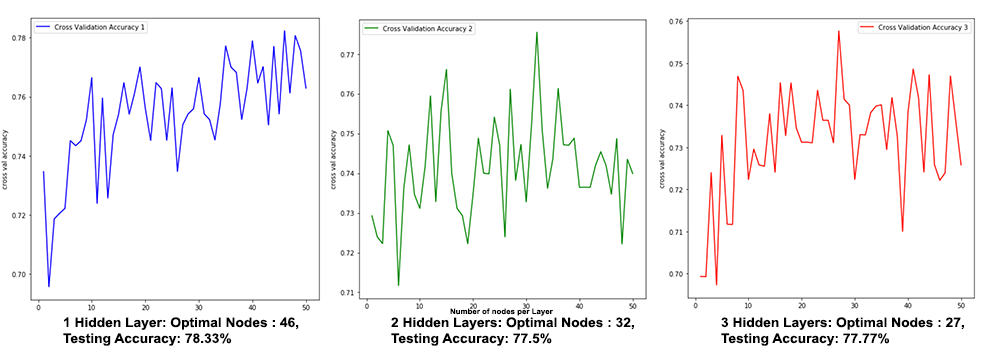
\includegraphics[scale = .50]{graph}
\caption{Figure2: ouput of predictive accuracy for 1,2 and 3 layer ANN's} 
\end{figure}

\subsection{Testing Code Functionality}
NEED TO TALK ABOUT UNIT TESTING . \\
Whilst developing each class and the functions associated with their respective classes, I generated a very small set of static data, an \textit{optimal} function, and the outputs of the data if the data was fed into this function. \\
The first class that was developed was the GenMember class to generate valid mathematical expressions, select parents, and update the population. After \textit{generate\textunderscore expression} was created, the only way to check this function was working was to run the function with a small depth e.g. \textit{gen\textunderscore depth=2}, and write out on a piece of paper who validate whether or not the function was creating different expressions each time the function was called with the generation depth imposed. To ensure that the \textit{get\textunderscore valid\textunderscore expression} worked, since the generated expression needed to contain all five variables X1,...X5, the only way that this condition could be checked was to call the function multiple times based on the generation created originally, and the new generation that fulfilled this condition, therefore, albeit an expression such as 'X1+6-X2+X3'/10*3 was a syntactically valid function, this is not considered to be a valid member within the population, however, an individual such as 'X1+X2-X3*X4/2+X5'  would be accepted, which would then be part of the original population as it met both the criteria. Using this, I extracted six generated members and their fitness values as this was all that was needed to allow the rest of the genetic program to function. To select the parents via tournament selection, all 6 of these members were inputted to the function. Based on my selection size, I was able to see that 'n' individuals were selected randomly. This was rerun multiple times to ensure that the same candidates were not chosen each time. \\
The next section to test was the ToPrefixParser class. To enable the infix to prefix conversion to work, the state of the infix expression had to be changed, such that it would be in an acceptable format for the \textit{get\textunderscore prefix\textunderscore notation} would accept. To initially test that the code that I used worked, I took one of the expressions and manually converted this to prefix notation, such that I knew that this expression was correct in the new state. Since I had the input and expected output, I was able to see if the functions associated with converting a simple expression from infix to prefix worked. Once this assertion was true, I then did repeated the process multiple times with expressions of varying sizes and bracketing, to see whether this infix to prefix converter was able to handle complex infix expressions with multiple numbers, variables and operators. Since \textit{get\textunderscore prefix\textunderscore notation} accepted an infix expression in the form "['X1','+','3']", I created the function \textit{split\textunderscore parents} to split the infix notation into the appropriate format. To test this worked, I fed in an expression to check whether or not the list was split into a format that \textit{get\textunderscore prefix\textunderscore notation} would accept. \\
Using two expressions that were converted into prefix, I was then able to start testing the \textit{Tree} class. Similar to how I tested whether the  \textit{get\textunderscore prefix\textunderscore notation} function worked, to test the  \textit{make\textunderscore tree}, I used a simple prefix expression, and manually constructed what the tree should look like based on the simple prefix expression given. As this was the expected tree, I was able to feed in the simple prefix expression and print the tree to the terminal. If the tree followed the same structure i.e. placed in the correct place, and also had the correct associations with their respective parents, then the \textit{make\textunderscore tree} function was functioning correctly. Based on the physical construction of the tree, and the node ID's that had been assigned to each node, after the output was produced, I was able to access each item in the tree and return their node value. If all the node values matched my construction, then I could assert that the tree was built correctly. This same process was repeated for larger, more complex prefix expressions, to ensure that this function could build any tree, based on any variety of prefix expression.  To ensure that \textit{find\textunderscore subtree} was performing as it should, rather than using a random node ID to find, I chose a specific node to find, such that I was able to perform the search manually and in a 'verbose' mode, such that as the function was running, I could confirm that at every stage, it was reaching the expected node that it was meant to, and eventually finding the appropriate node which could then be returned. Another crucial function that needed to work at all times, was \textit{swap\textunderscore nodes}. To be able to test this, I used two two prefix expressions that were definitely in the correct form when being represented in their binary tree structure. By inserting and printing the parents that would be crossed over, it was obvious to see that the nodes had been changed before and after the crossover took place. The reason this was easy is that I was able to print the new trees produced and compare the original parents to the children, based on the child nodes that I had selected to be crossed over.  This same process was performed for the \textit{mutate\textunderscore node} function, as they both required the trees, and the node to be manipulated, therefore since I selected a specific node to be mutated, I was able to see exactly what it was mutated to, to ensure that this function was performing as expected.\\
The next class that needed testing was the \textit{ToInfixParser} class.  To test this class, using a simple problem to begin with, I used a basic binary tree that was created, and placed into the appropriate formatted list of nodes which could then be passed into the function. Though writing down what should be the expected output, and running the function, I was able to show that the function was able to produce the expected output that I had created manually. After this, I was able to use the expression produced to test if the \textit{conv\textunderscore inf} function was able to map the prefix expression back into the correct infix expression.  To test this function, as every sub expression produced would be encapsulated in parentheses, I then had to evaluate the infix expression so that I could ensure that although the structure may be different, the output was still the same.  

\subsection{Running the Genetic Program - Training and Testing datasets}

In genetic programming, to allow the network to learn and find patterns in the data to try to produce an optimal solution, the network has to be trained. This means 
During the development of the program, after the main program was created, it was recommended that the dataset that I had should be split into two datasets such that I could train the network to a certain degree of accuracy, and then use another dataset that could be used to test the predictive accuracy of an unknown dataset. \\
Rather than training the dataset on a large amount of data and testing it on another large dataset, I extracted 10 rows of data from the proper dataset, and used this to train the network. After the network was sufficiently trained, for example, if it reached a certain fitness level for the dataset given or if the program reached the maximum iteration criteria, then the current best solution would be returned as well as the predictive accuracy of the GP that was trained to get the best solution.  As the \textit{optimal solution} was found, I then took another row of data from the dataset (which had not been a part of the initial 10 rows being used for training) and inserted the testing test data row into the optimal equation. The evaluated value was then passed through a sigmoid function, as this was used to represent the data between a range of 0 and 1, and was used to determine which class the company fell into . If the value produced by the sigmoidal function was below 0.499, then the company was classed as "not likely to fail", however if it was 0.5 and above, the company was classified as "likely to fail".\\

My first method of testing was to train the GP using the full given data set. After this was done, since I had no other dataset, I used the same dataset to test the predictive accuracy of the genetic program optimal equations. Using the 

One the project was completed, using the leave one out technique, I removed one of the rows of data from the dataset, which could be used as a testing row. This technique is known as the  \textit{leave one out} method. Here, the training dataset is every single row other than one, which is used as the testing dataset. The problem with this method is that if the GP overfits the data, then just because the testing prediction is correct, this could have happened entirely through chance. If the GP overfits the data, then when using a bigger dataset for prediction, generalisation will be worse, which will produce a worse prediction result as the data has been poorly generalised. \\

Another model evaluation procedure was then used to estimate how well the GP would perform on a set of testing data. 
\subsection{Testing Selection Methods}
\subsection{Paramater Tuning}

\subsection{evaluation of ANN and GP }
\newpage
\section{Comparisons of Artificial Neural Networks and Genetic Programs}
\newpage
\section{Critical assessment of the project }
\subsection{What was Successful}

\newpage
\section{Future Work}
\subsection{Possible Improvements}

\newpage
\section{Conclusion}







\end{document}


